\section{Vetores}

Existem dois tipos de grandezas: \textbf{escalares} e \textbf{vetoriais}.

As grandezas \textbf{escalares} são completamente definidas por um número real
acompanhado de uma unidade adequada, como comprimento, volume e temperatura.

Já as grandezas \textbf{vetoriais} necessitam de três elementos para sua
completa definição:

\begin{itemize}
    \item \textbf{Módulo}: intensidade do vetor;
    \item \textbf{Direção}: determinada por uma reta e todas as suas paralelas
    (Figura~\ref{fig:fig1.1a});
    \item \textbf{Sentido}: indica para onde o vetor aponta em sua direção
    (Figura~\ref{fig:fig1.1b}).
\end{itemize}

\begin{figure}[H]
    \centering
    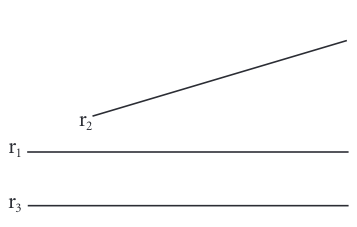
\includegraphics[width=0.5\textwidth]{./fig/fig1.1a.png}
    \caption{Direção de um vetor}\label{fig:fig1.1a}
\end{figure}

\begin{figure}[H]
    \centering
    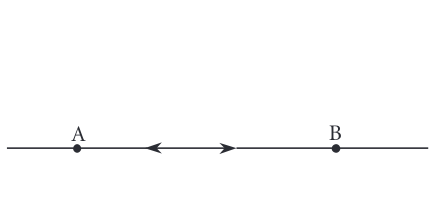
\includegraphics[width=0.5\textwidth]{./fig/fig1.1b.png}
    \caption{Sentido de um vetor}\label{fig:fig1.1b}
\end{figure}

\subsection{Representação de Vetores}

Um vetor pode ser representado por um \textbf{segmento orientado}, onde:
\begin{itemize}
    \item O \textbf{módulo} é o comprimento do segmento;
    \item A \textbf{direção} é definida pelo ângulo do vetor;
    \item O \textbf{sentido} é indicado pela extremidade do segmento
      (Figura~\ref{fig:fig1.2}).
\end{itemize}

\begin{figure}[H]
    \centering
    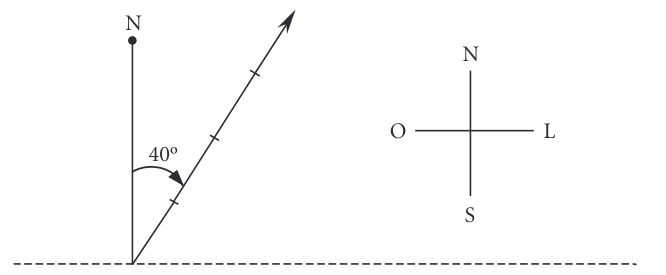
\includegraphics[width=0.5\textwidth]{./fig/fig1.2.png}
    \caption{Representação de um vetor}\label{fig:fig1.2}
\end{figure}

Dois vetores com mesmo comprimento, mesma direção e mesmo sentido são
equivalentes (Figura~\ref{fig:fig1.3}). Isso significa que um vetor pode ser
\textbf{transladado} para qualquer ponto do espaço sem alterar suas
propriedades, sendo chamado de \textbf{vetor livre} (Figura~\ref{fig:fig1.4}).

\begin{figure}[H]
    \centering
    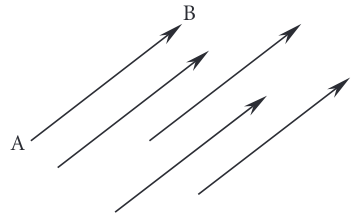
\includegraphics[width=0.5\textwidth]{./fig/fig1.3.png}
    \caption{Vetores equivalentes}\label{fig:fig1.3}
\end{figure}

\begin{figure}[H]
    \centering
    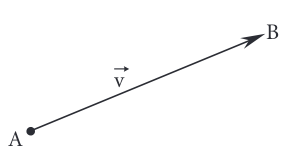
\includegraphics[width=0.5\textwidth]{./fig/fig1.4.png}
    \caption{Vetor livre}\label{fig:fig1.4}
\end{figure}

\subsection{Casos Particulares de Vetores}
\begin{itemize}
    \item \textbf{Vetores paralelos} ($\mathbf{u} // \mathbf{v}$): possuem a
    mesma direção (Figura~\ref{fig:fig1.6}).
    \begin{figure}[H]
        \centering
        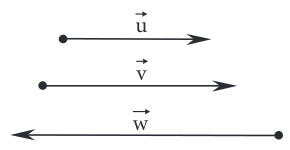
\includegraphics[width=0.5\textwidth]{./fig/fig1.6.png}
        \caption{Vetores paralelos}\label{fig:fig1.6}
    \end{figure}
    \item \textbf{Vetores iguais} ($\mathbf{u} = \mathbf{v}$): possuem mesmo
    módulo, direção e sentido.
    \item \textbf{Vetor nulo} ($\mathbf{0}$): não possui direção nem sentido
    definidos e é paralelo a qualquer vetor.
    \item \textbf{Vetores opostos} ($-\mathbf{v}$): mesma direção e módulo, mas
    sentidos contrários (Figura~\ref{fig:fig1.7}).
    \begin{figure}[H]
        \centering
        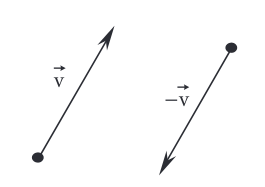
\includegraphics[width=0.5\textwidth]{./fig/fig1.7.png}
        \caption{Vetores opostos}\label{fig:fig1.7}
    \end{figure}
    \item \textbf{Vetor unitário (versor)}: possui módulo igual a 1
      (Figura~\ref{fig:fig1.8}).
    \begin{figure}[H]
        \centering
        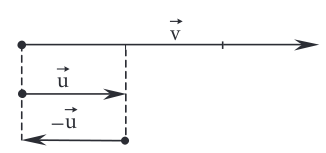
\includegraphics[width=0.5\textwidth]{./fig/fig1.8.png}
        \caption{Versor de um vetor}\label{fig:fig1.8}
    \end{figure}
    \item \textbf{Vetores ortogonais} ($\mathbf{u} \perp \mathbf{v}$): formam um
    ângulo reto entre si (Figura~\ref{fig:fig1.9}).
    \begin{figure}[H]
        \centering
        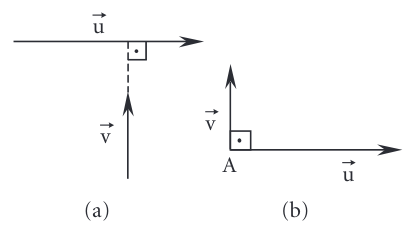
\includegraphics[width=0.5\textwidth]{./fig/fig1.9.png}
        \caption{Vetores ortogonais}\label{fig:fig1.9}
    \end{figure}
    \item \textbf{Vetores coplanares}: pertencem ao mesmo plano
      (Figuras~\ref{fig:fig1.10} e~\ref{fig:fig1.11}).
    \begin{figure}[H]
        \centering
        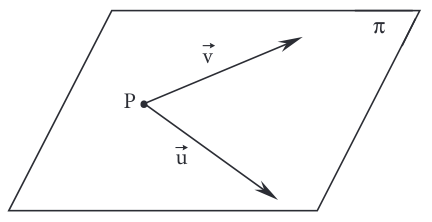
\includegraphics[width=0.5\textwidth]{./fig/fig1.10.png}
        \caption{Vetores coplanares (caso 1)}\label{fig:fig1.10}
    \end{figure}
    
    \begin{figure}[H]
        \centering
        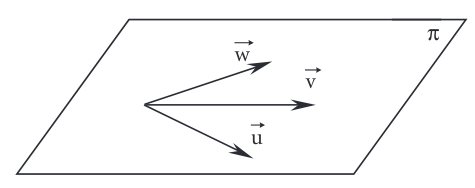
\includegraphics[width=0.5\textwidth]{./fig/fig1.11.png}
        \caption{Vetores coplanares (caso 2)}\label{fig:fig1.11}
    \end{figure}
\end{itemize}

\newpage

\subsection{Exemplos}

\question{
A Figura~\ref{fig:fig1.12} é constituída de nove quadrados congruentes (de mesmo
tamanho). Decidir se é verdadeira ou falsa cada uma das seguintes afirmações:
}
\begin{figure}[H]
    \centering
    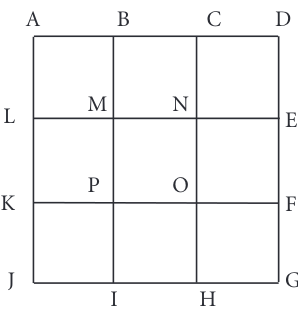
\includegraphics[width=0.5\textwidth]{./fig/fig1.12.png}
    \caption{}\label{fig:fig1.12}
\end{figure}
\begin{center}
% First column
\begin{minipage}[t]{0.24\textwidth}
\begin{itemize}
  \item \subquestion{$\overrightarrow{\mathrm{AB}} = \overrightarrow{\mathrm{OF}}$} \answer{V}
  \item \subquestion{$\overrightarrow{\mathrm{AM}} = \overrightarrow{\mathrm{PH}}$} \answer{V}
  \item \subquestion{$\overrightarrow{\mathrm{BC}} = \overrightarrow{\mathrm{OP}}$} \answer{F}
  \item \subquestion{$\overrightarrow{\mathrm{BL}} = \overrightarrow{\mathrm{MC}}$} \answer{F}
  \item \subquestion{$\overrightarrow{\mathrm{DE}} = -\overrightarrow{\mathrm{ED}}$} \answer{V}
\end{itemize}
\end{minipage}
\hfill
% Second column
\begin{minipage}[t]{0.24\textwidth}
\begin{itemize}
  \item \subquestion{$\overrightarrow{\mathrm{AO}} = \overrightarrow{\mathrm{MG}}$} \answer{V}
  \item \subquestion{$\overrightarrow{\mathrm{KN}} = \overrightarrow{\mathrm{FI}}$} \answer{V}
  \item \subquestion{$\overrightarrow{\mathrm{AC}} \parallel \overrightarrow{\mathrm{HI}}$} \answer{V}
  \item \subquestion{$\overrightarrow{\mathrm{JO}} \parallel \overrightarrow{\mathrm{LD}}$} \answer{F}
  \item \subquestion{$\overrightarrow{\mathrm{AJ}} \parallel \overrightarrow{\mathrm{FG}}$} \answer{V}
\end{itemize}
\end{minipage}
\hfill
% Third column
\begin{minipage}[t]{0.24\textwidth}
\begin{itemize}
  \item \subquestion{$\overrightarrow{\mathrm{AB}} \perp \overrightarrow{\mathrm{EG}}$} \answer{V}
  \item \subquestion{$\overrightarrow{\mathrm{AM}} \perp \overrightarrow{\mathrm{BL}}$} \answer{V}
  \item \subquestion{$\overrightarrow{\mathrm{PE}} \perp \overrightarrow{\mathrm{EC}}$} \answer{F}
  \item \subquestion{$\overrightarrow{\mathrm{PN}} \perp \overrightarrow{\mathrm{NB}}$} \answer{V}
  \item \subquestion{$\overrightarrow{\mathrm{PN}} \perp \overrightarrow{\mathrm{AM}}$} \answer{V}
\end{itemize}
\end{minipage}
\hfill
% Fourth column
\begin{minipage}[t]{0.24\textwidth}
\begin{itemize}
  \item \subquestion{$|\overrightarrow{\mathrm{AC}}| = |\overrightarrow{\mathrm{FP}}|$} \answer{V}
  \item \subquestion{$|\overrightarrow{\mathrm{IF}}| = |\overrightarrow{\mathrm{MF}}|$} \answer{V}
  \item \subquestion{$|\overrightarrow{\mathrm{AJ}}| = |\overrightarrow{\mathrm{AC}}|$} \answer{F}
  \item \subquestion{$|\overrightarrow{\mathrm{AO}}| = 2|\overrightarrow{\mathrm{NP}}|$} \answer{V}
  \item \subquestion{$|\overrightarrow{\mathrm{AM}}| = |\overrightarrow{\mathrm{BL}}|$} \answer{V}
\end{itemize}
\end{minipage}
\end{center}

\newpage

\question{
A Figura~\ref{fig:fig1.13} representa um paralelepípedo retângulo. Decidir se é
verdadeira ou falsa cada uma das afirmações:
}
\begin{figure}[H]
    \centering
    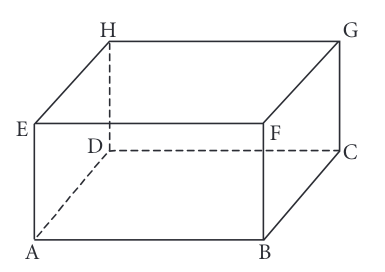
\includegraphics[width=0.5\textwidth]{./fig/fig1.13.png}
    \caption{}\label{fig:fig1.13}
\end{figure}
\begin{center}
% First column
\begin{minipage}[t]{0.24\textwidth}
\begin{itemize}
  \item \subquestion{$\overrightarrow{\mathrm{DH}} = \overrightarrow{\mathrm{BF}}$} \answer{V}
  \item \subquestion{$\overrightarrow{\mathrm{AB}} = -\overrightarrow{\mathrm{HG}}$} \answer{F}
  \item \subquestion{$\overrightarrow{\mathrm{AB}} \perp \overrightarrow{\mathrm{CG}}$} \answer{V}
  \item \subquestion{$\overrightarrow{\mathrm{AF}} \perp \overrightarrow{\mathrm{BC}}$} \answer{V}
\end{itemize}
\end{minipage}
\hfill
% Second column
\begin{minipage}[t]{0.24\textwidth}
\begin{itemize}
  \item \subquestion{|$\overrightarrow{\mathrm{AC}}| = |\overrightarrow{\mathrm{HF}}|$} \answer{V}
  \item \subquestion{|$\overrightarrow{\mathrm{AG}}| = |\overrightarrow{\mathrm{DF}}|$} \answer{V}
  \item \subquestion{$\overrightarrow{\mathrm{BG}} \parallel \overrightarrow{\mathrm{ED}}$} \answer{F}
  \item \subquestion{$\overrightarrow{\mathrm{AB}} \text{, } \overrightarrow{\mathrm{BC}} \text{ e } \overrightarrow{\mathrm{CG}} \\
    \text{ são coplanares }$} \answer{F}
\end{itemize}
\end{minipage}
\hfill
% Third column
\begin{minipage}[t]{0.24\textwidth}
\begin{itemize}
  \item \subquestion{$\overrightarrow{\mathrm{AB}} \text{, } \overrightarrow{\mathrm{FG}} \text{ e } \overrightarrow{\mathrm{EG}} \\
    \text{ são coplanares }$} \answer{V}
  \item \subquestion{$\overrightarrow{\mathrm{EG}} \text{, } \overrightarrow{\mathrm{CB}} \text{ e } \overrightarrow{\mathrm{HF}} \\
    \text{ são coplanares }$} \answer{V}
  \item \subquestion{$\overrightarrow{\mathrm{AC}} \text{, } \overrightarrow{\mathrm{DB}} \text{ e } \overrightarrow{\mathrm{FG}} \\
    \text{ são coplanares }$} \answer{V}
  \item \subquestion{$\overrightarrow{\mathrm{AB}} \text{, } \overrightarrow{\mathrm{BG}} \text{ e } \overrightarrow{\mathrm{CF}} \\
    \text{ são coplanares }$} \answer{F}
\end{itemize}
\end{minipage}
\hfill
% Fourth column
\begin{minipage}[t]{0.24\textwidth}
\begin{itemize}
  \item \subquestion{$\overrightarrow{\mathrm{AB}} \text{, } \overrightarrow{\mathrm{DC}} \text{ e } \overrightarrow{\mathrm{CF}} \\
    \text{ são coplanares }$} \answer{V}
  \item \subquestion{$\overrightarrow{\mathrm{AE}} \text{ é ortogonal ao plano } \\
    ABC$} \answer{V}
  \item \subquestion{$\overrightarrow{\mathrm{AV}} \text{ é ortogonal ao plano } \\
    BCG$} \answer{V}
  \item \subquestion{$\overrightarrow{\mathrm{DC}} \text{ é paralelo ao plano } \\
    HEF$} \answer{V}
\end{itemize}
\end{minipage}
\end{center}
